\documentclass[12pt, twoside]{article}
\usepackage[francais]{babel}
\usepackage[T1]{fontenc}
\usepackage[latin1]{inputenc}
\usepackage[left=5mm, right=5mm, top=5mm, bottom=5mm]{geometry}
\usepackage{float}
\usepackage{graphicx}
\usepackage{array}
\usepackage{multirow}
\usepackage{amsmath,amssymb,mathrsfs}
\usepackage{soul}
\usepackage{textcomp}
\usepackage{eurosym}
 \usepackage{variations}
\usepackage{tabvar}


\pagestyle{empty}

\begin{document}


\section*{\center{Devoir maison 5}}


\bigskip


\begin{center}
\fbox{


\textit{Devoir � rendre pour le \textbf{mercredi 5 f�vrier 2014}. L'exercice 4
est � faire sur la photocopie.}

}


\end{center}


\bigskip


\ul{Exercice 1}: (\textit{2 points}) 


\begin{enumerate}
  \item Construire la figure en vraie grandeur.
  \item Quelle est la nature du triangle ABC?
\end{enumerate}


\bigskip

\ul{Exercice 2}: (\textit{4 points}) 

\begin{enumerate}
  \item Placer deux points M et N distants de 4,5 cm. 
  \item Tracer le cercle $\mathcal{C}_1$ de centre N passant par M.
\item Tracer le cercle $\mathcal{C}_2$ de centre M de rayon 4,5 cm. Les
cercles $\mathcal{C}_1$  et $\mathcal{C}_2$ se coupent en deux points Y et Z.
\item Sans mesurer, donner en justifiant la distance NY.
\item Que peut-on dire du quadrilat�re MYNZ? Justifier. 
\end{enumerate}

\bigskip

 
\ul{Exercice 3}: (\textit{5.5 points})

\begin{enumerate}
  \item Construire un triangle RJZ tel RJ=5,5cm ; JZ=4cm et ZR=6cm.
  \item Tracer la m�diatrice (d) du segment [RZ]. Elle coupe la droite (RJ) au
  point S.
  \item Placer un point U qui appartienne � la droite (d). Quelle est la nature
  du triangle URZ? Expliquer votre r�ponse.
  \item Tracer la droite parall�le � (RZ) passant par S.
\end{enumerate}

\bigskip

\ul{Exercice 4}: (\textit{8.5 points}) \qquad \textbf{Le tr�sor de l'�le aux
requins \ldots}

\enskip


Il y a tr�s longtemps, des corsaires ont cach� sur cette �le \textbf{deux
tr�sors}: un premier coffre contenant 120 diamants et un deuxi�me coffre
contenant 3500 pi�ces d'or.

Julie a trouv� un document qui va lui permettre de trouver les emplacements des
deux tr�sors: aide la � utiliser ces renseignements:

\begin{enumerate}
 \item 
  
  \begin{enumerate}
    
    
  \item Une premi�re bouteille  est enterr�e sur l'�le. Cette bouteille
  est align�e avec la grotte et la source. Elle est aussi align�e avec l'arbre
 pench� et le phare. \textbf{On appelle B l'emplacement de cette bouteille.
 Placer ce point B sur la carte}.
  \item Dans cette bouteille se trouve le renseignement suivant: ``Le coffre
  contenant les diamants est � 0,3 km du gros rocher et � 0,5 km de la
  tour''.
  \textbf{On appelle C l'emplacement du coffre de diamants. Placer ce point C
  sur la carte.}
  \end{enumerate}
  
  \item 
  
  \begin{enumerate}
    \item Une deuxi�me bouteille est enterr�e � 850 m du phare et � �gales
    distances de l'arbre pench� et du gros rocher. \textbf{On appelle B'
    l'emplacement de la deuxi�me bouteille. Placer ce point B' sur la carte}.
    \item Dans cette bouteille se trouve le renseignement suivant: ``Le coffre
    contenant les pi�ces d'or est enterr� � 0,3 km du gros rocher et � 0,5 km de
    la tour, mais il n'est pas avec le coffre contenant les diamants.''
    \textbf{On appelle C' l'emplacement du deuxi�me coffre. Placer ce point C'
    sur la carte.}
    
    \end{enumerate}
\end{enumerate}
 
 \pagebreak
 
 
 
NOM PRENOM: \ldots \ldots \ldots \ldots \ldots\ldots

 
\begin{center}
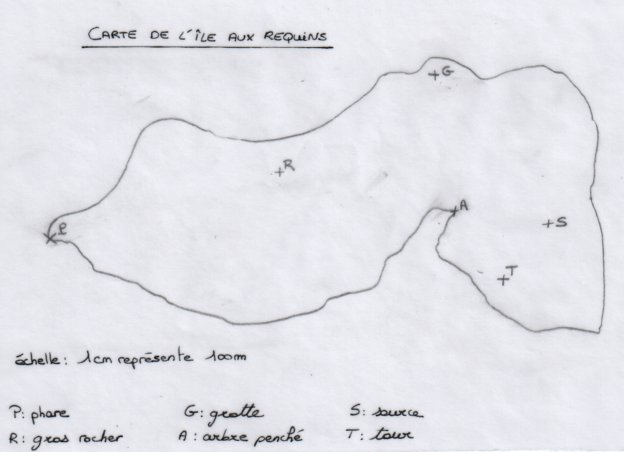
\includegraphics[width=17cm]{images/carte.jpg} 
\end{center}

\bigskip



\bigskip

NOM PRENOM: \ldots \ldots \ldots \ldots \ldots\ldots


\begin{center}
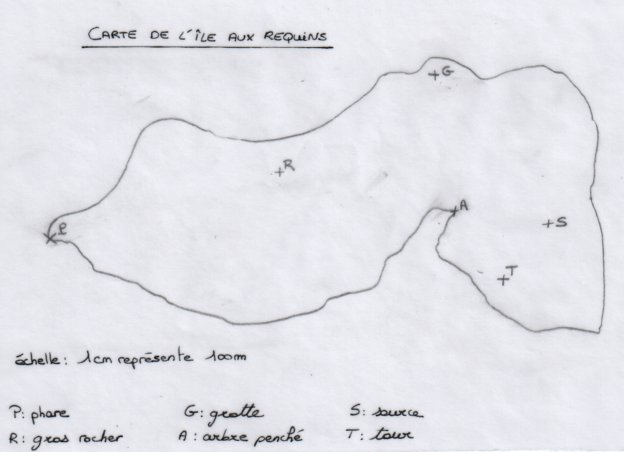
\includegraphics[width=17cm]{images/carte.jpg} 
\end{center}
\end{document}
